\chapter{Experimental Evaluation} \label{chap:results}

The account of the research should be presented in a manner suitable for the field. It should be complete, systematic, and sufficiently detailed to enable a reader to understand how the data were gathered and how to apply similar methods in another study. Notation and formatting must be consistent throughout the thesis, including units of measure, abbreviations, and the numbering scheme for tables, figures, footnotes, and citations. One or more chapters may consist of material published (or submitted for publication) elsewhere. See “Including Published Material in a Thesis or Dissertation” for details.

\section{Verification of the Network Implementation}

\section{Terrain Processing Results}

\subsection{Analysis of Terrain Similarity} \label{ssec:terrains_analysis}
In the following a brief analysis of terrain similarities is presented. In general, a (dis-) similarity between terrains should correlate with classification results, i.e., the more two terrains differ from each other the better classification results are expected, and vice versa.

In order to quantify and visualise similarity among various terrains, a similarity measure was calculated as given in \cref{eq:similarity_measure}. The five qualities are listed in \cref{tab:terrain_features} and in \cref{tab:terrains_parameters}.

\begin{align} \label{eq:similarity_measure}
  SM_{t_1, t_2} = \frac{\displaystyle\sum_{i=1}^{5} \abs{quality(i, t_1) - quality(i, t_2)}}{5}
\end{align} 

The similarity measure equals 0 if two terrains are identical (have the same parameter values) and equals 1.0 if two terrains are totally different.

The following \cref{fig:terrain_similarity_measures} shows the similarity measures among generated terrains.

\begin{figure}[H]
  \centering
  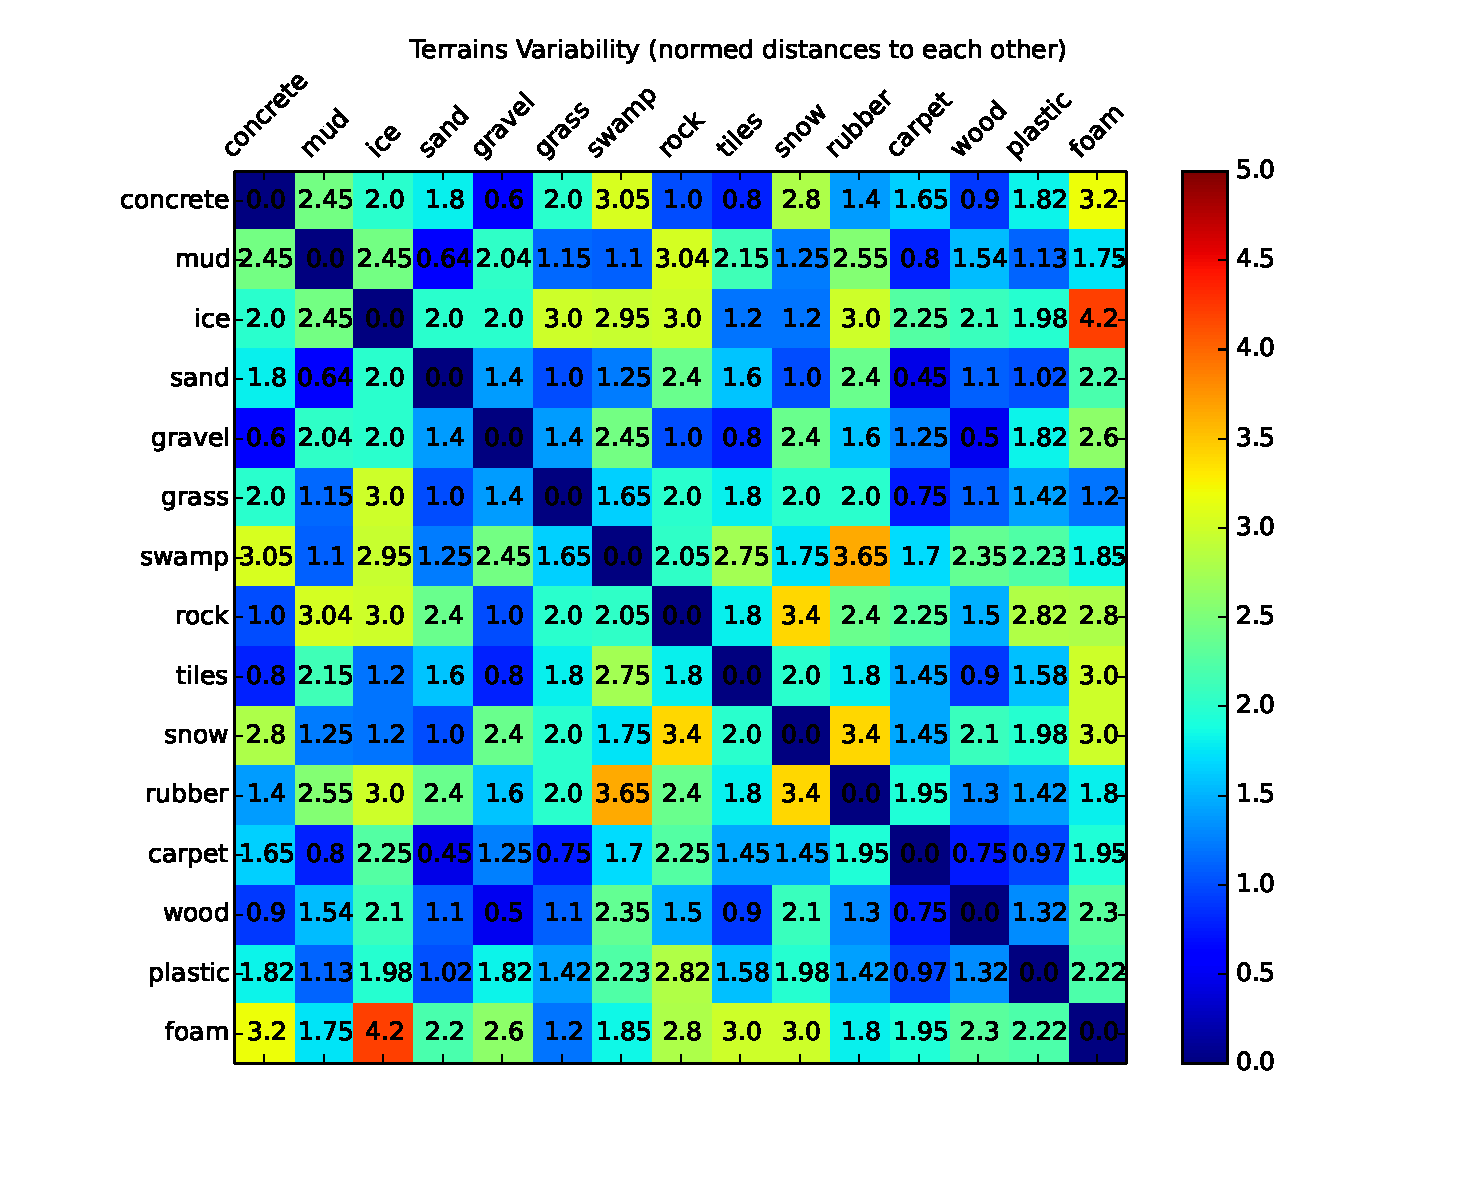
\includegraphics[width=1.0\textwidth]{terrains_variability.eps}
  \caption{Similarity measures among various terrain types.}
  \label{fig:terrain_similarity_measures}
\end{figure}

The surfaces have been generated virtually and their similarity to real world terrains has not been verified. However, results demonstrate that foam is very different from ice or, for instance, sand is quite similar to mud. A low similarity measure can be seen among concrete, carpet and rubber as all of them are moreless flat.

Surprisingly, a wooden terrain ended up as very similar to gravel and carpet, but a limited number of simulated terrain features has to be considered. 
On the other hand, rubber results as very different from swamp and snow, which is a positive outcome. Also the high grass-ice or rock-snow similarity measures make sense. 

\subsection{Gathered Data} \label{ssec:gathered_data}

\begin{figure}[H]
  \centering
  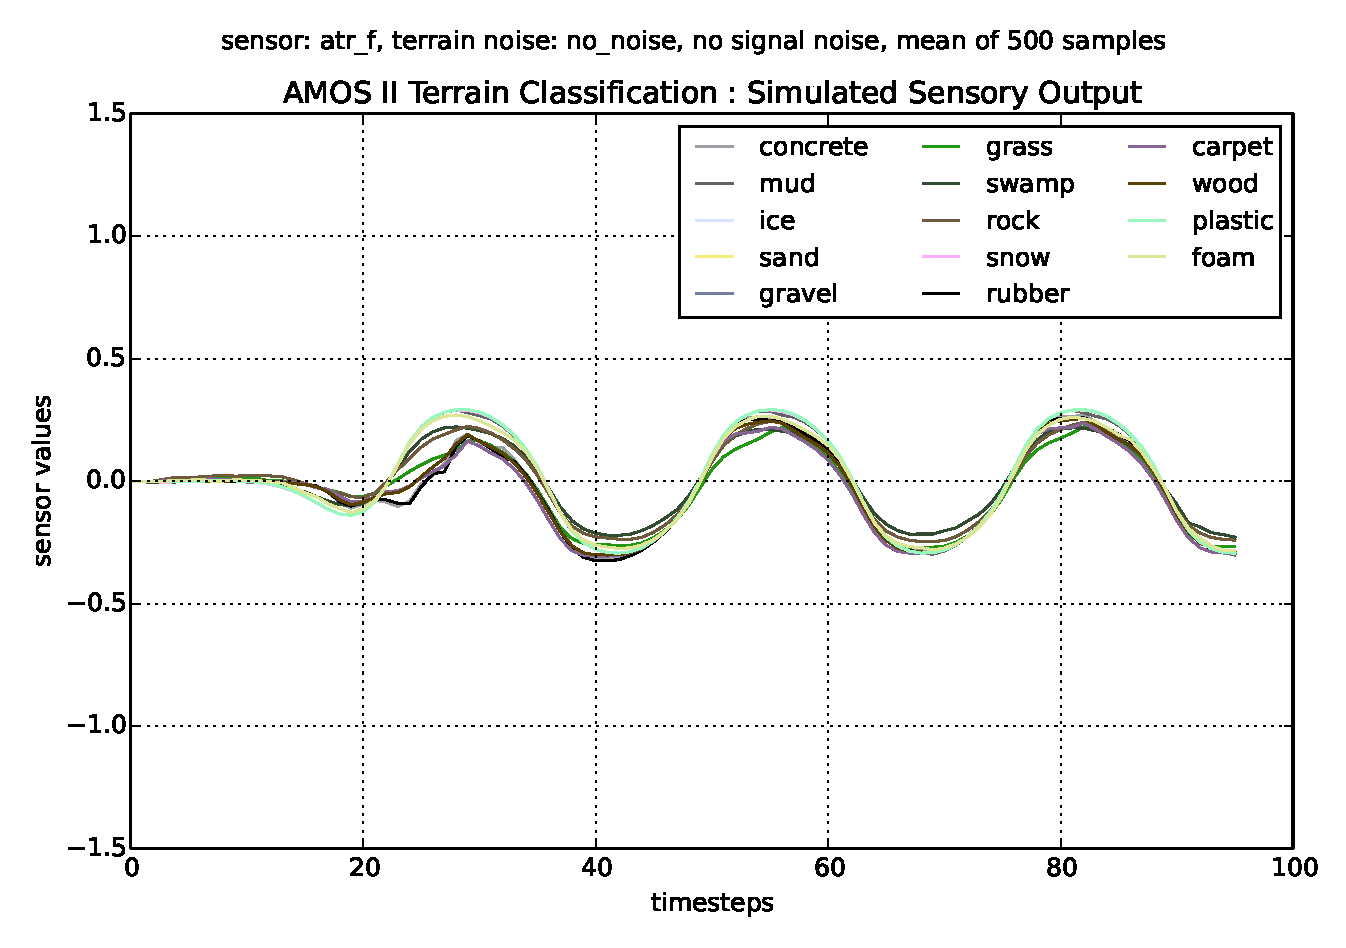
\includegraphics[width=1.0\textwidth]{sensor_atr_f_no_noise}
  \caption{Sensor ATRf : mean of 500 samples, 14 terrains}
  \label{fig:sensor_atr_f_no_noise}
\end{figure}

\begin{figure}[H]
  \centering
  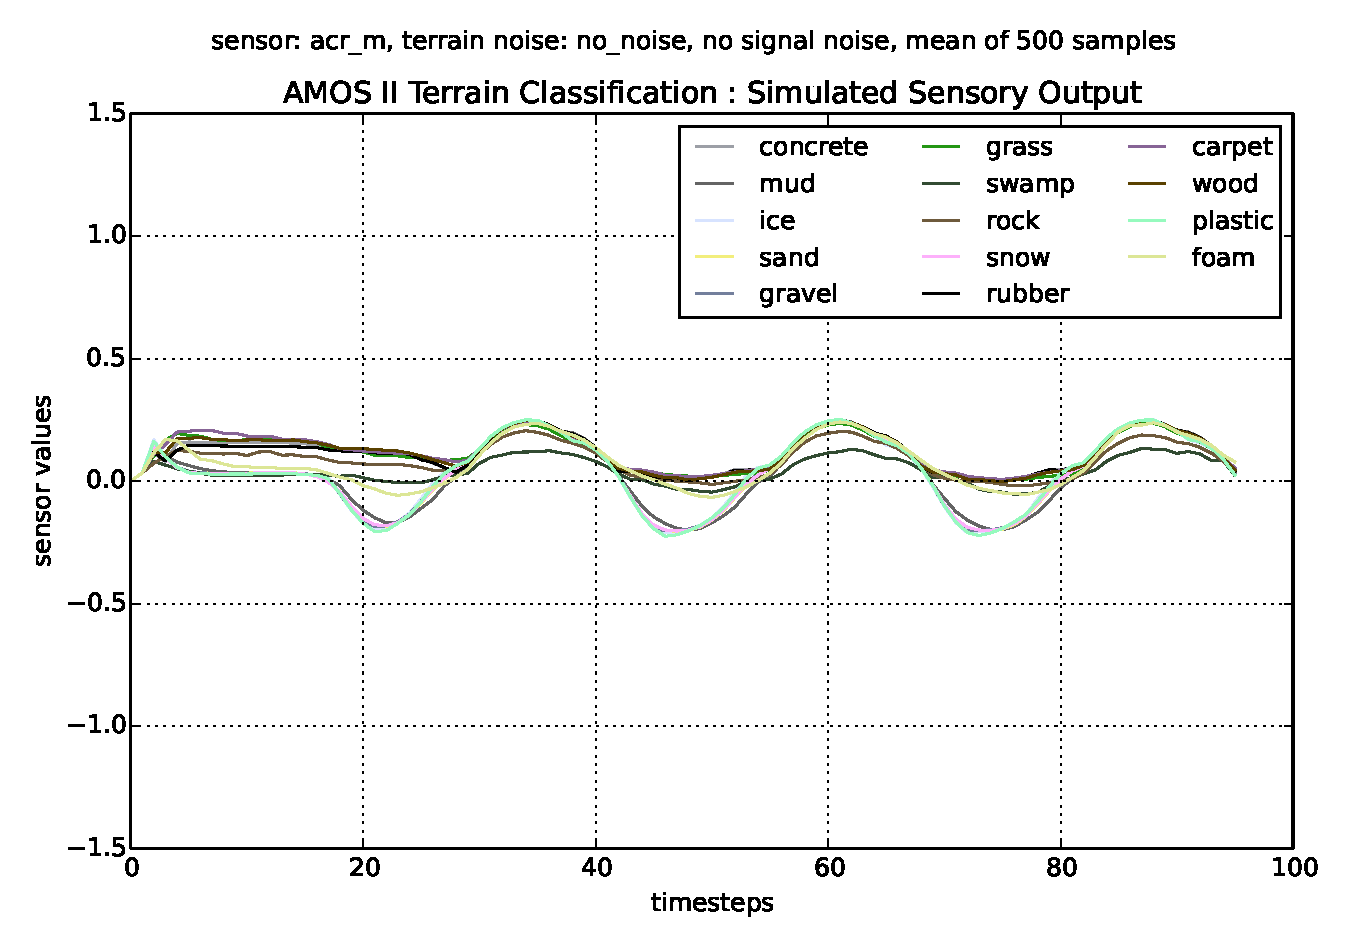
\includegraphics[width=1.0\textwidth]{sensor_acr_m_no_noise}
  \caption{Sensor ACRm : mean of 500 samples, 14 terrains}
  \label{fig:sensor_acr_m_no_noise}
\end{figure}

\begin{figure}[H]
  \centering
  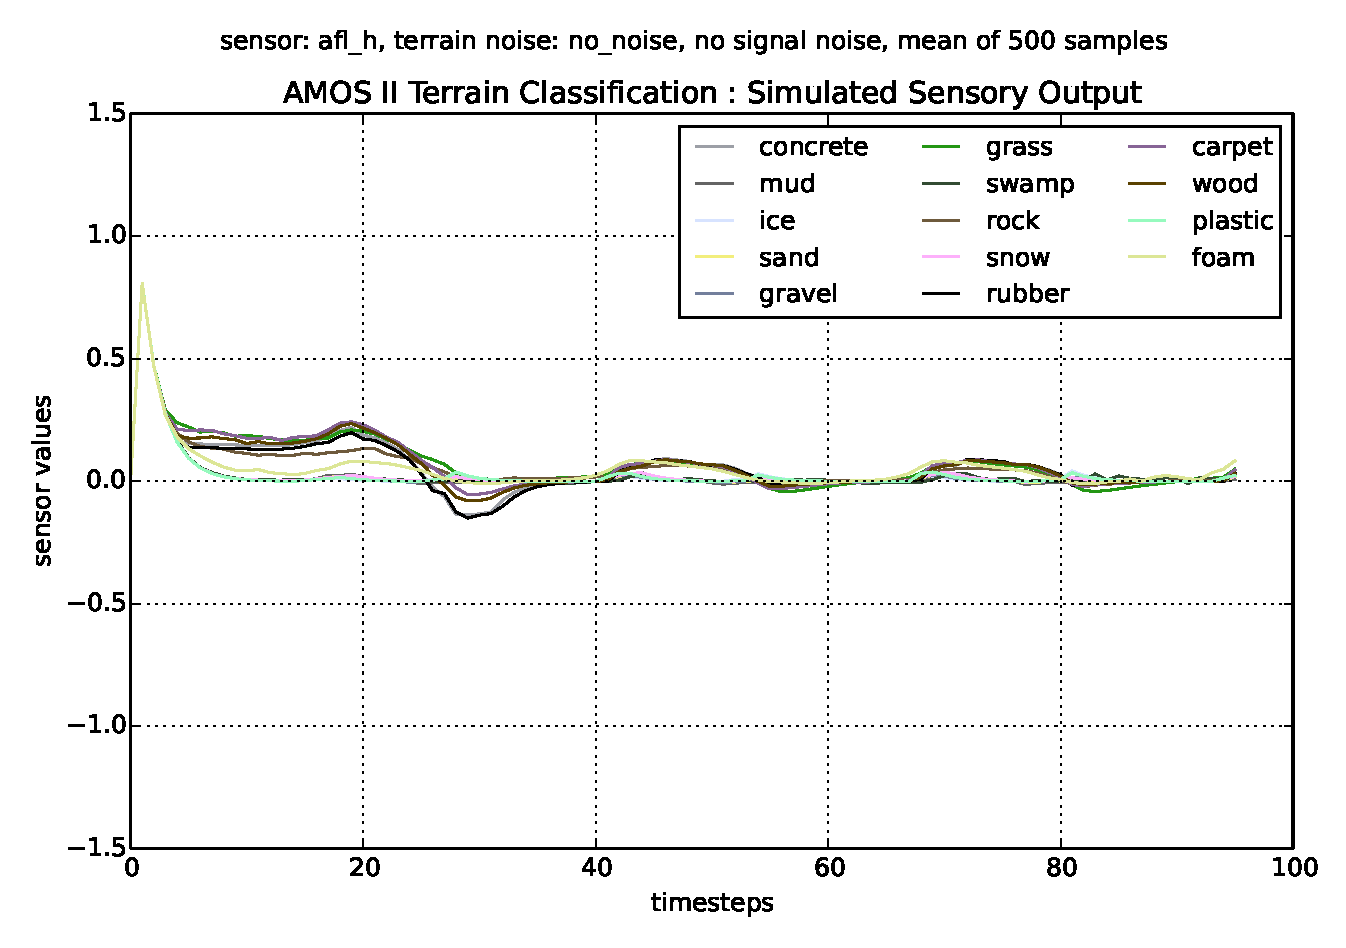
\includegraphics[width=1.0\textwidth]{sensor_afl_h_no_noise}
  \caption{Sensor AFLh : mean of 500 samples, 14 terrains}
  \label{fig:sensor_afl_h_no_noise}
\end{figure}

\begin{figure}[H]
  \centering
  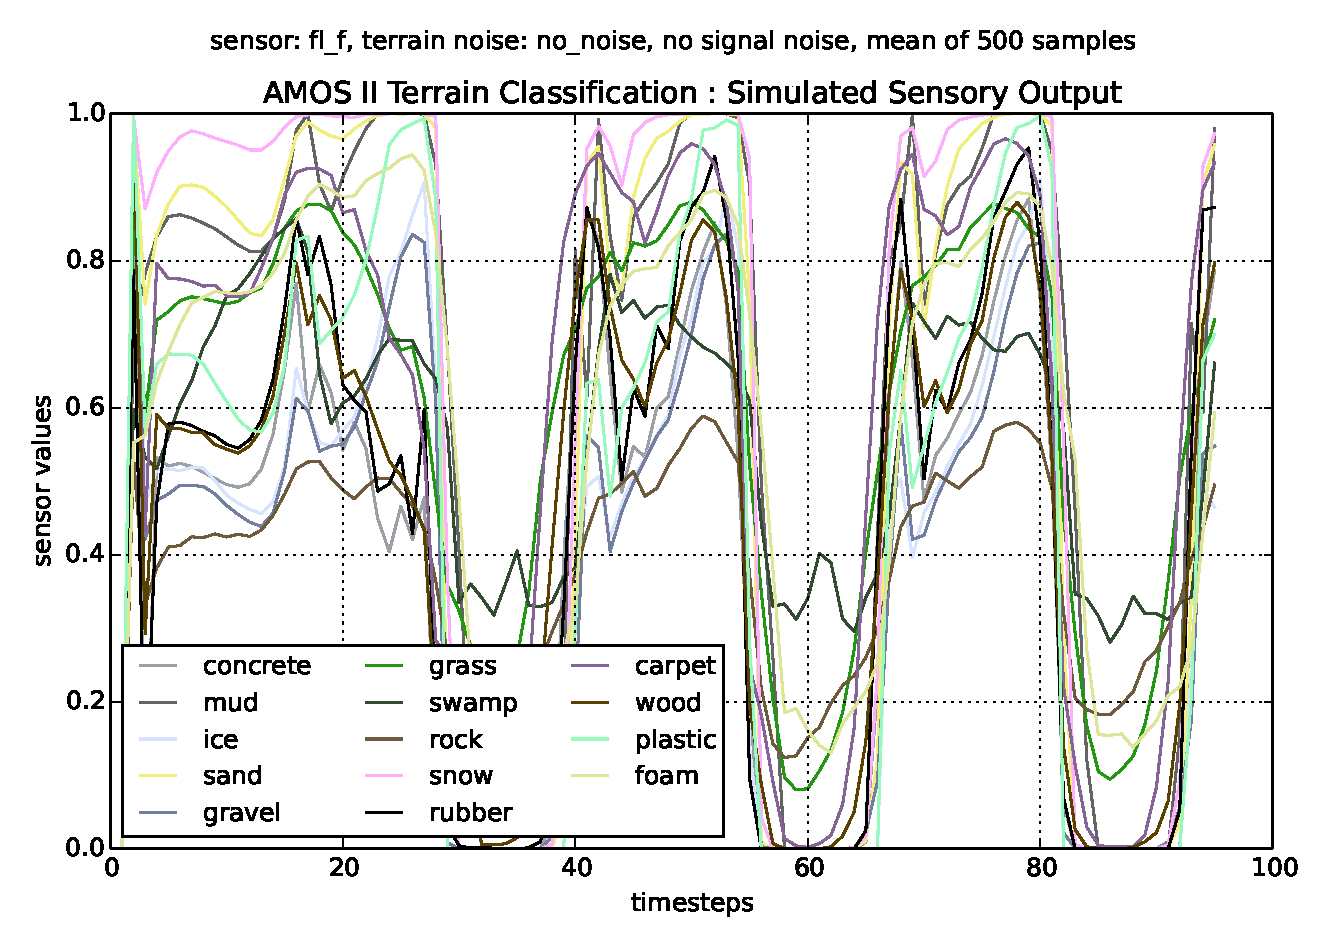
\includegraphics[width=1.0\textwidth]{sensor_fl_f_no_noise}
  \caption{Sensor FLf : mean of 500 samples, 14 terrains}
  \label{fig:sensor_fl_f_no_noise}
\end{figure}

\subsection{Built Feature Vector} \label{ssec:built_feature_vectors}

\begin{figure}[H]
  \centering
  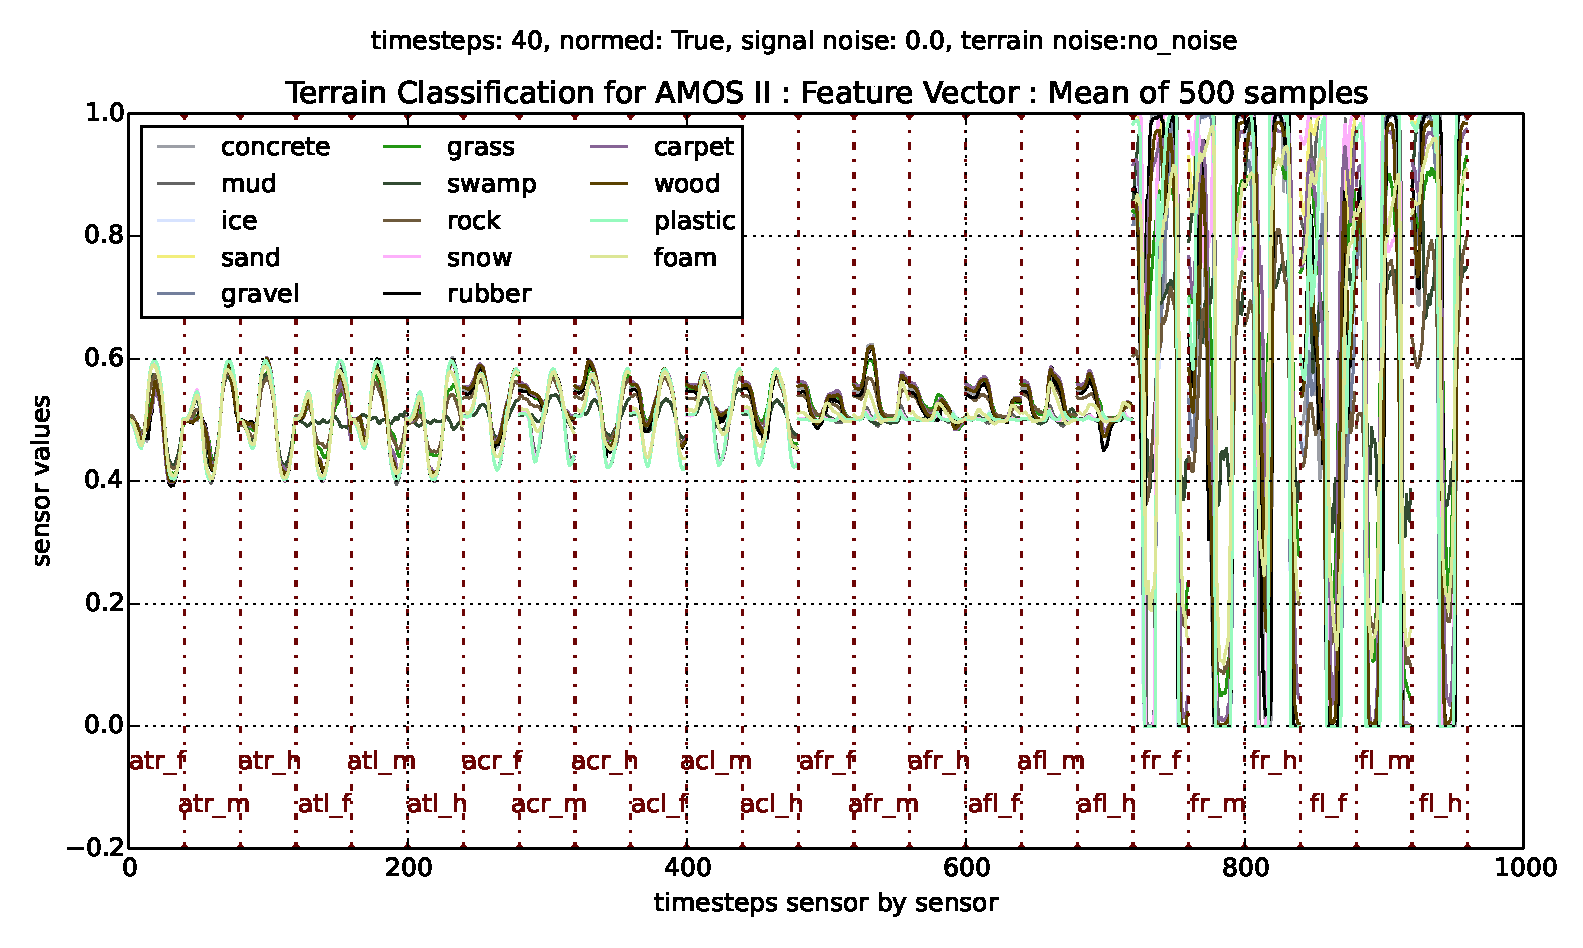
\includegraphics[width=1.0\textwidth]{sample_no_noise_0_40}
  \caption{Feature Vector : mean of 500 samples, 14 terrains, no noise, 40 timesteps}
  \label{fig:sample_40t}
\end{figure}


\begin{figure}[H]
  \centering
  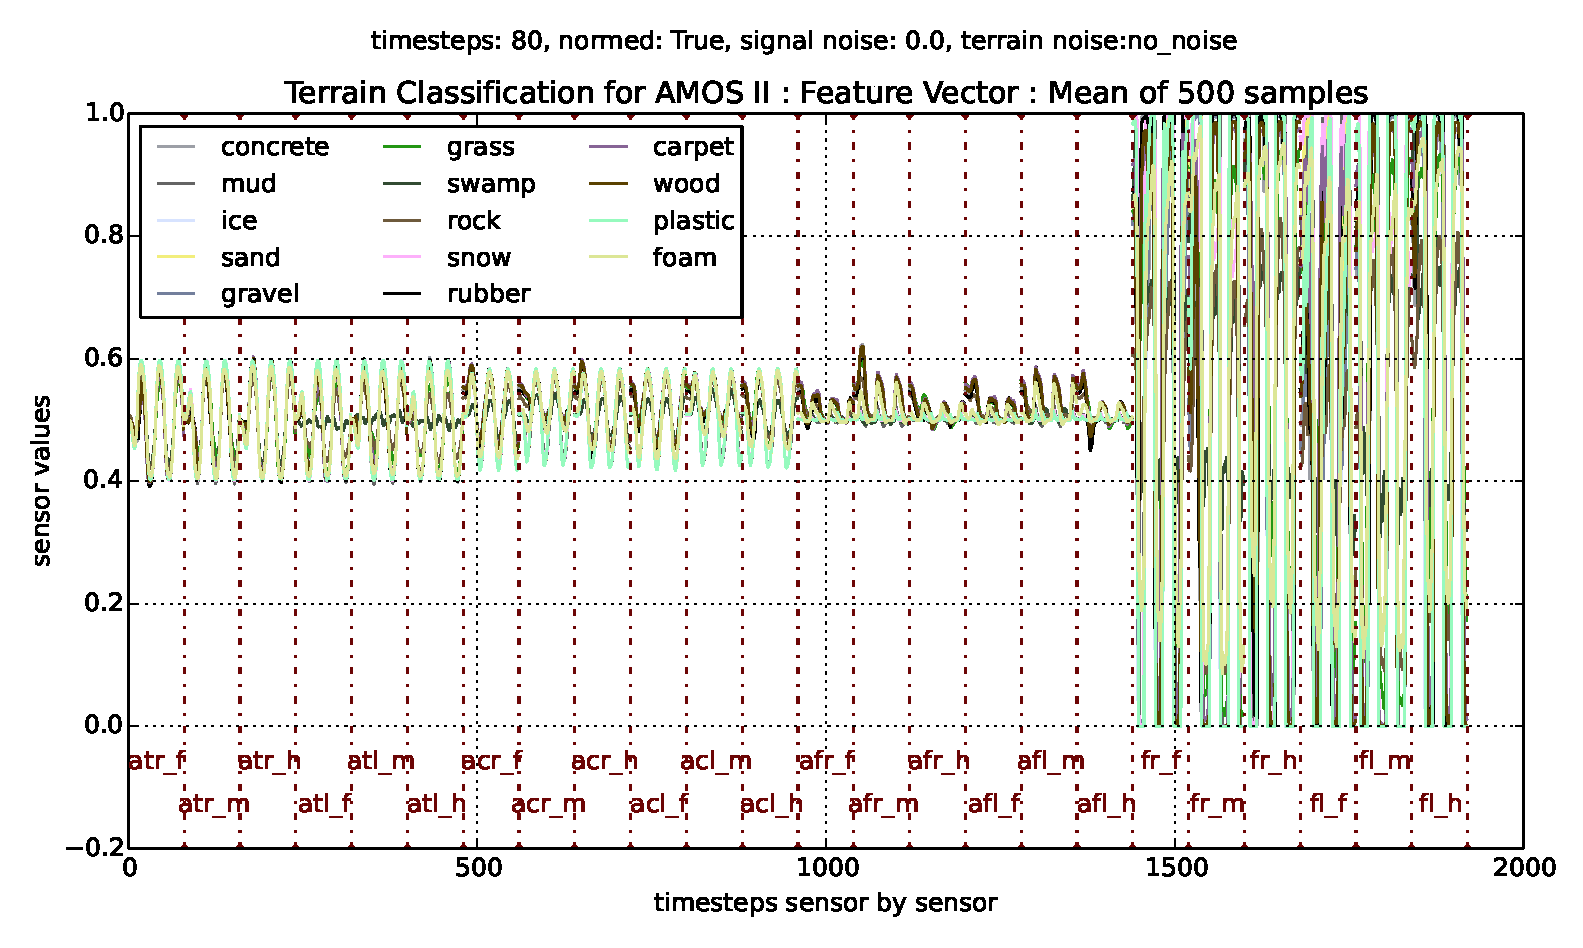
\includegraphics[width=1.0\textwidth]{sample_no_noise_0_80}
  \caption{Feature Vector : mean of 500 samples, 14 terrains, no noise, 80 timesteps}
  \label{fig:sample_80t}
\end{figure}

\subsection{Terrain Noise Influence} \label{ssec:terrain_noise_influence}

\begin{figure}[H]
  \centering
  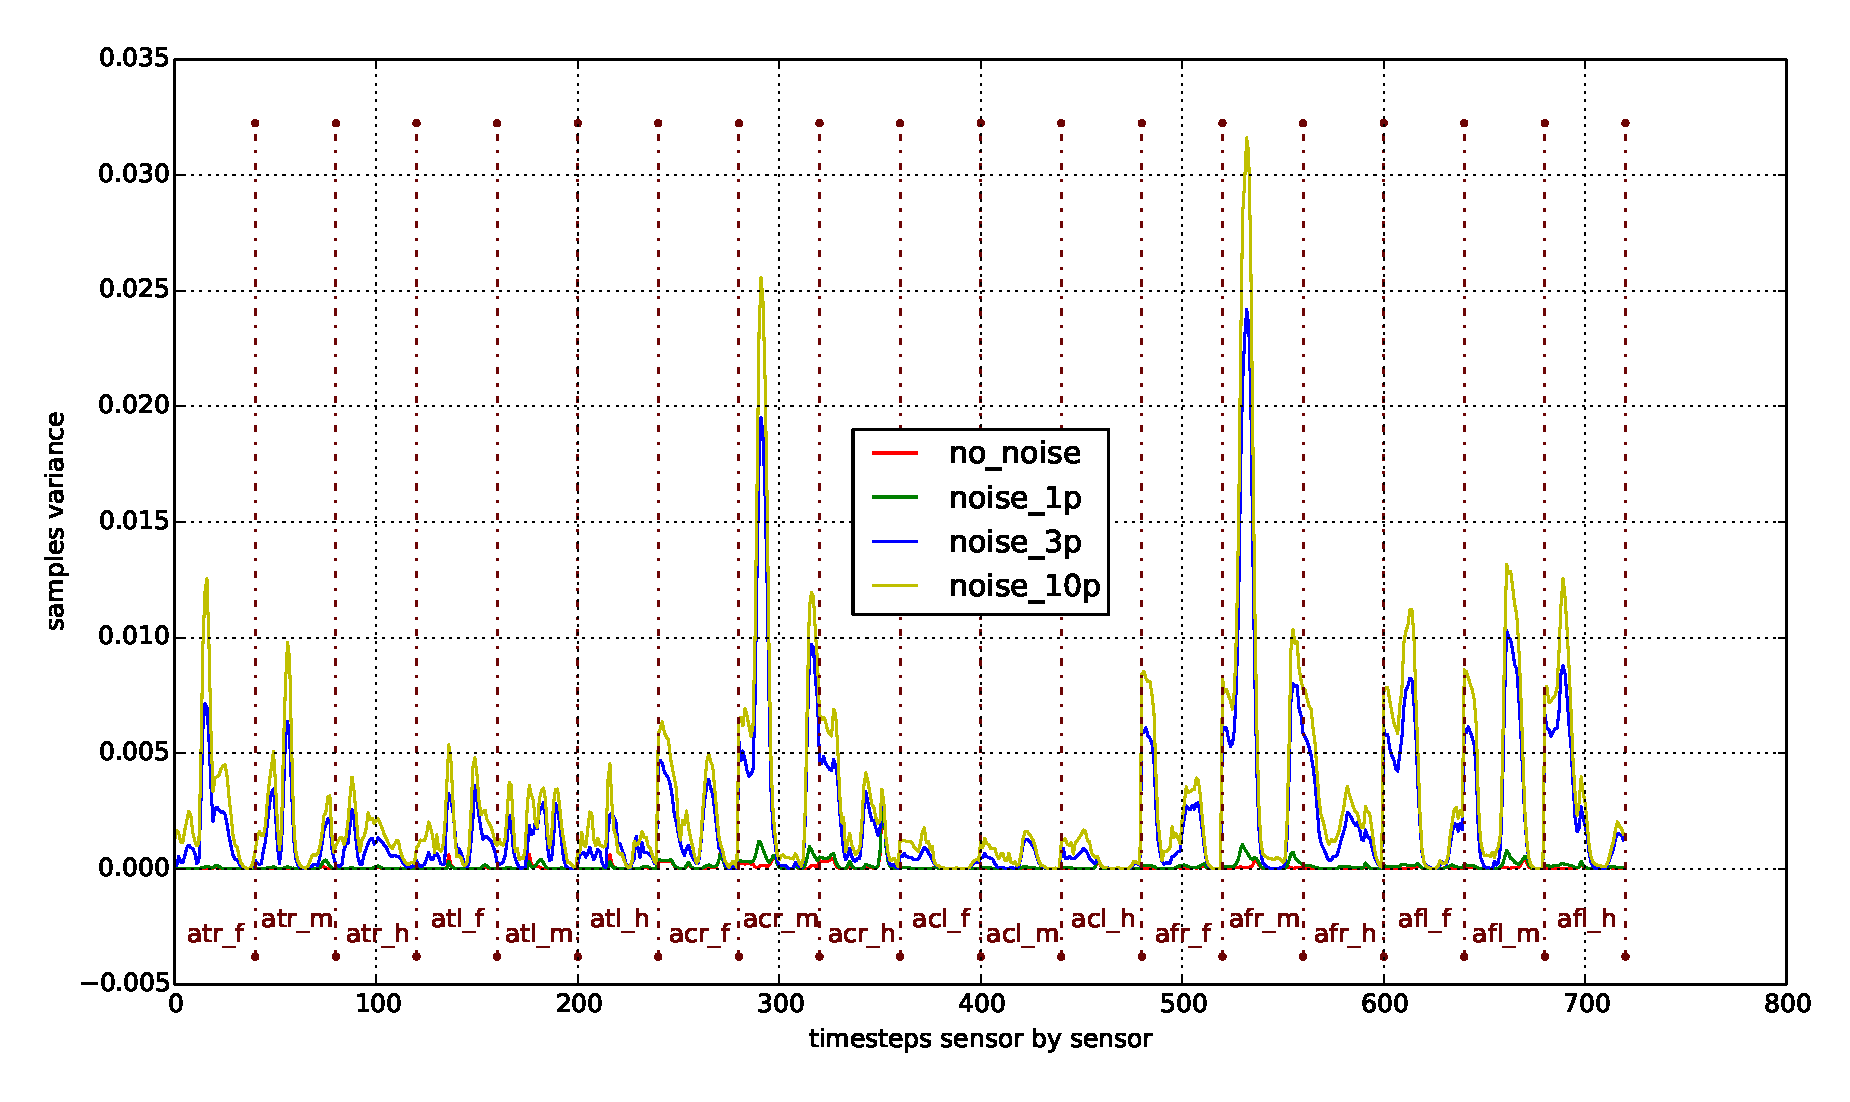
\includegraphics[width=1.0\textwidth]{tn_analysis_40_angle_gravel}
  \caption{Terrain Noise Analysis (samples variance): 500 samples, terrain gravel, angle sensors (feature vector [0:720] for 40 timesteps)}
  \label{fig:tn_analysis_angle_gravel}
\end{figure}

\begin{figure}[H]
  \centering
  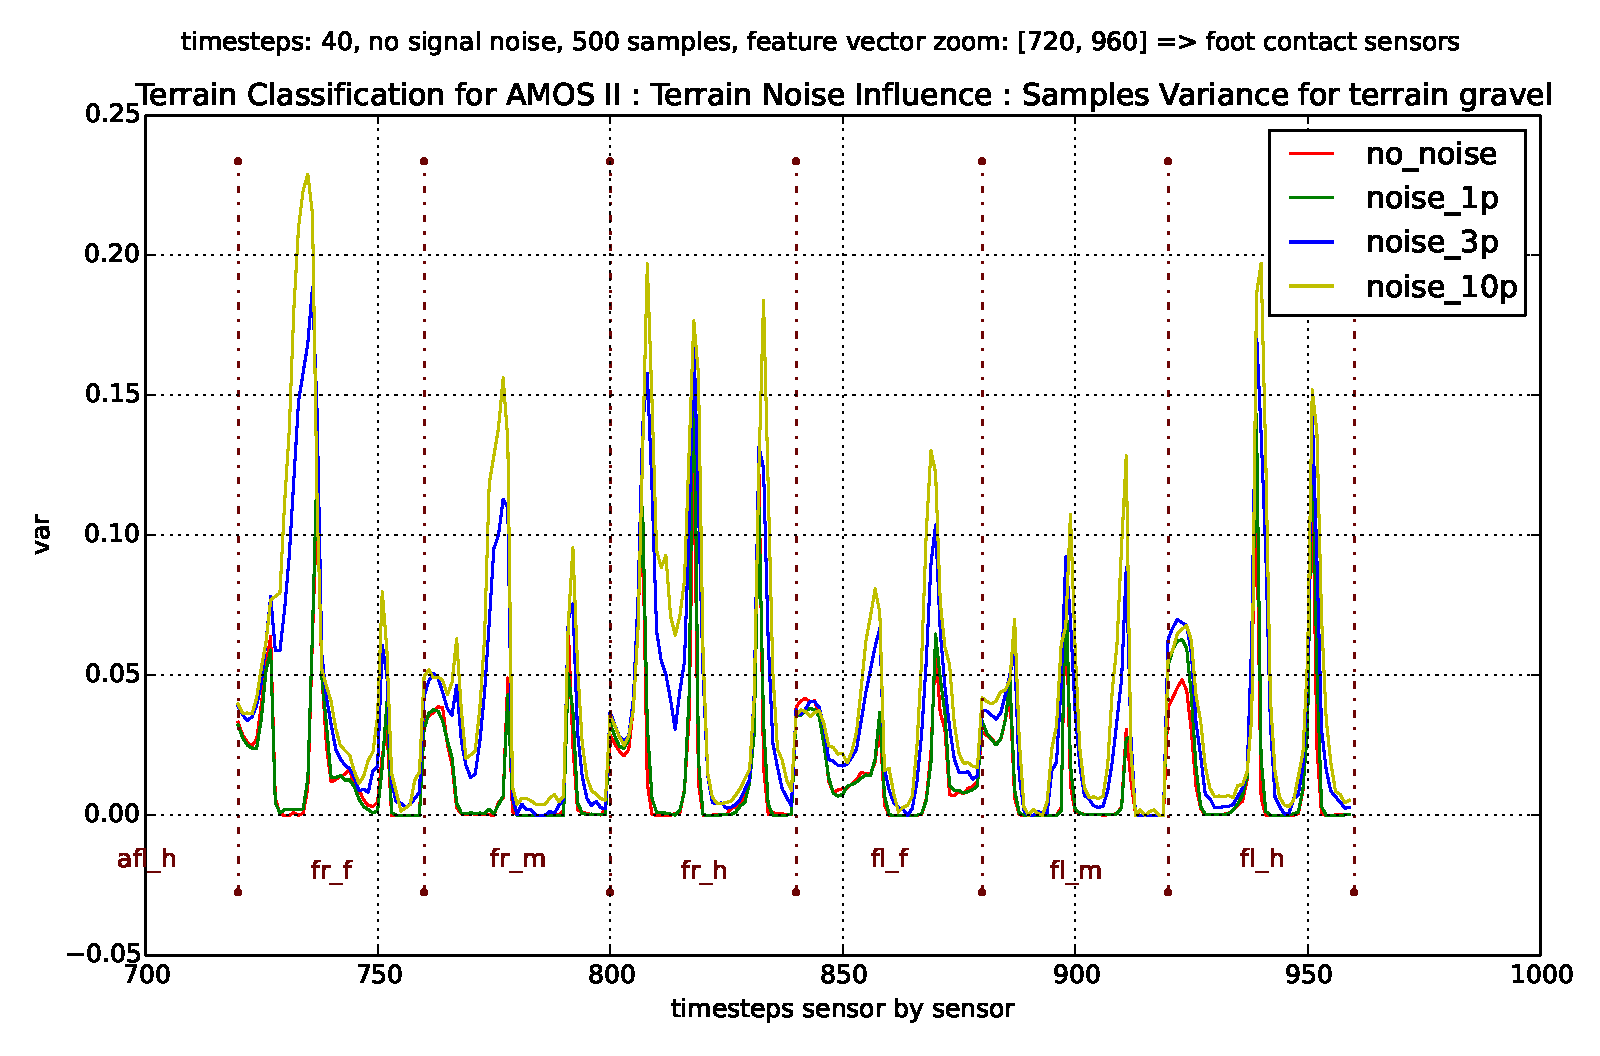
\includegraphics[width=1.0\textwidth]{tn_analysis_40_foot_contact_gravel}
  \caption{Terrain Noise Analysis (samples variance): 500 samples, terrain gravel, foot contact sensors (feature vector [720:960] for 40 timesteps)}
  \label{fig:tn_analysis_foot_contact_gravel}
\end{figure}

\begin{figure}[H]
  \centering
  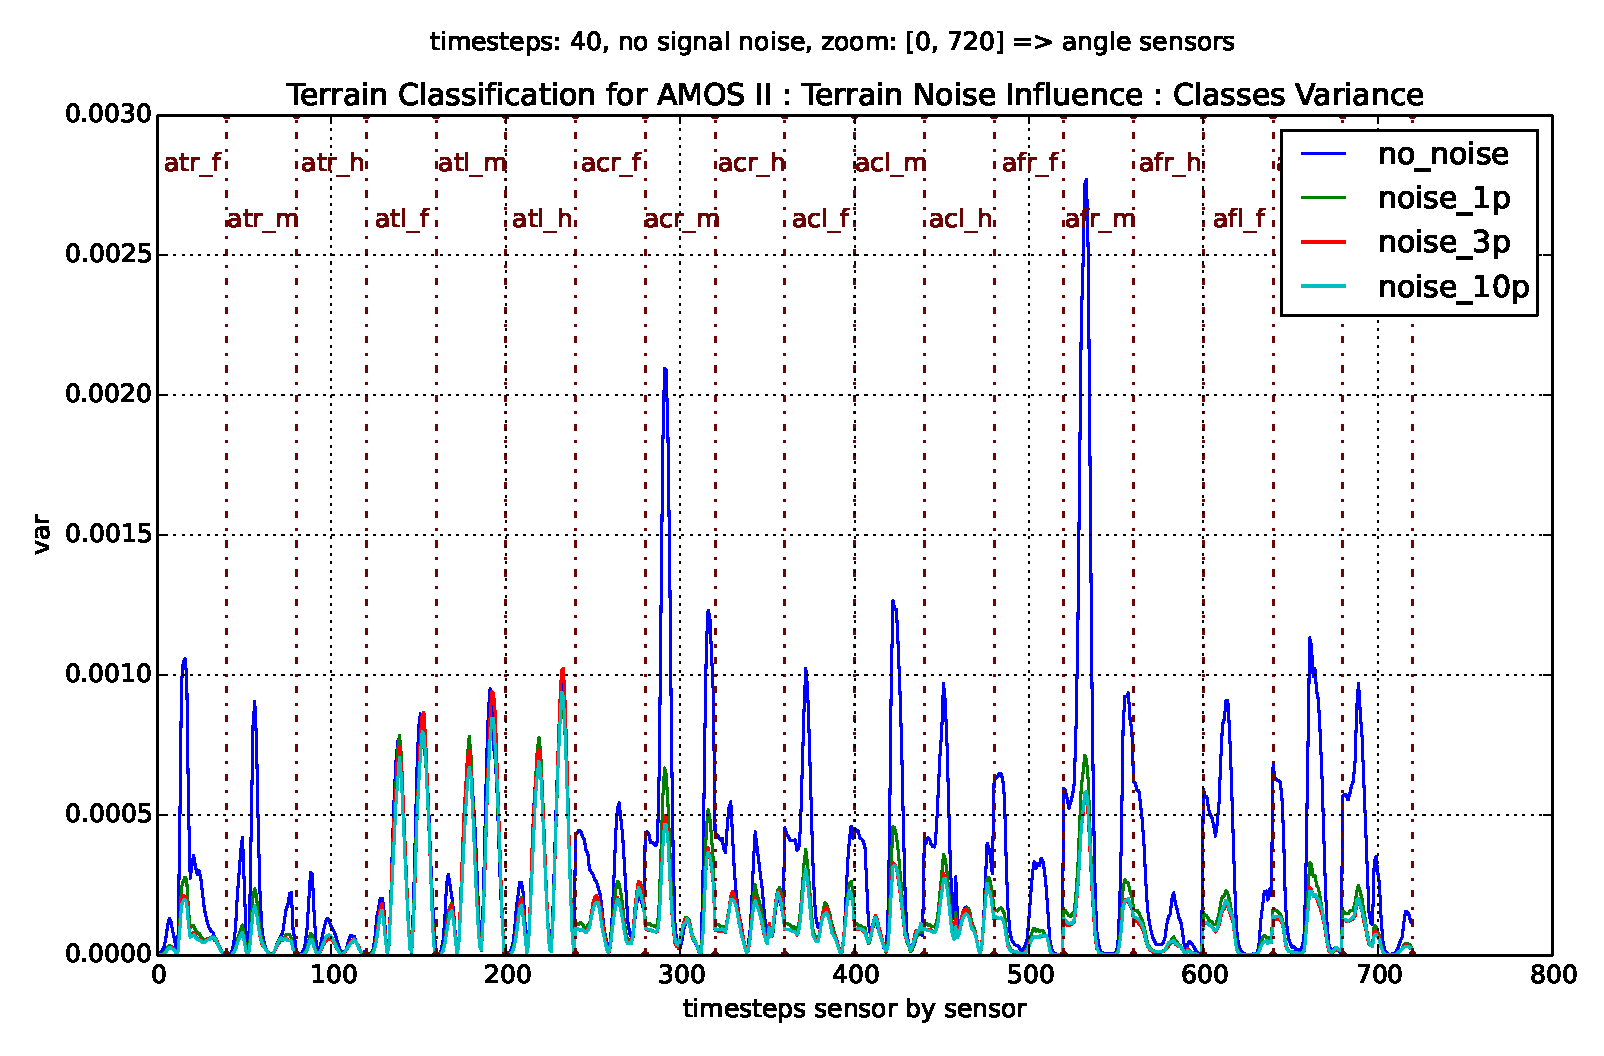
\includegraphics[width=1.0\textwidth]{tn_analysis_40_angle}
  \caption{Terrain Noise Analysis (classes variance): means of 500 samples, 14 terrains, angle sensors}
  \label{fig:tn_analysis_angle}
\end{figure}

\begin{figure}[H]
  \centering
  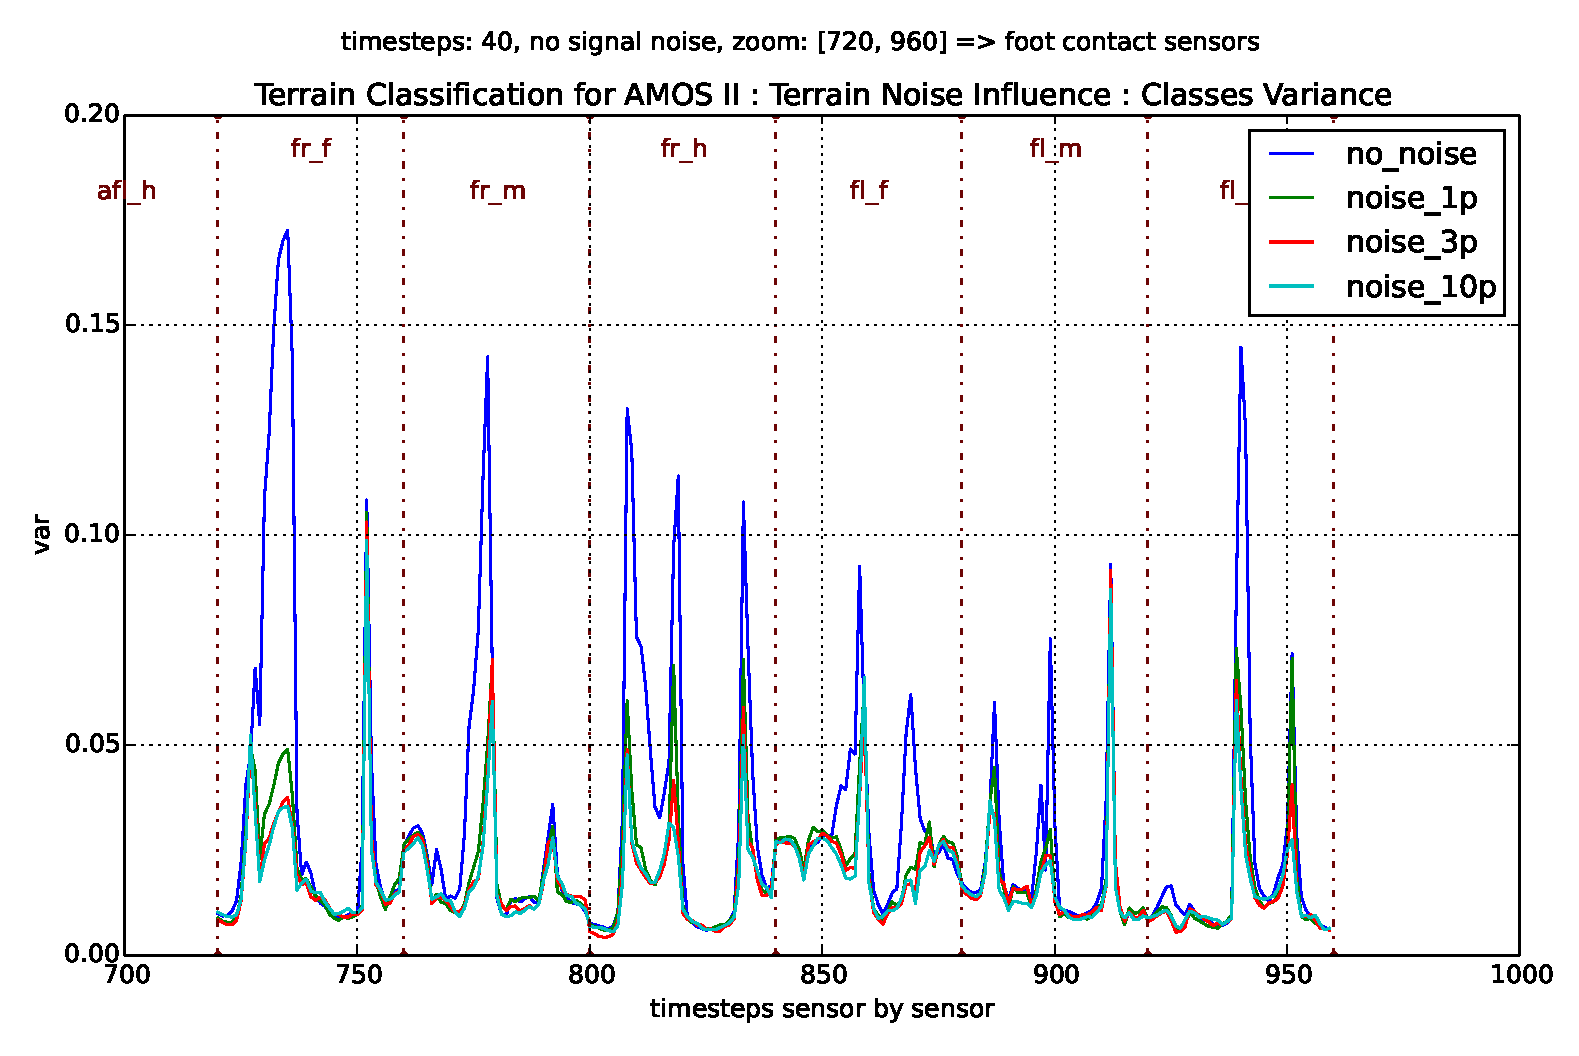
\includegraphics[width=1.0\textwidth]{tn_analysis_40_foot_contact}
  \caption{Terrain Noise Analysis (classes variance): means of 500 samples, 14 terrains, foot contact sensors}
  \label{fig:tn_analysis_foot_contact}
\end{figure}

\subsection{Signal Noise Influence} \label{ssec:signal_noise_influence}

\begin{figure}[H]
  \centering
  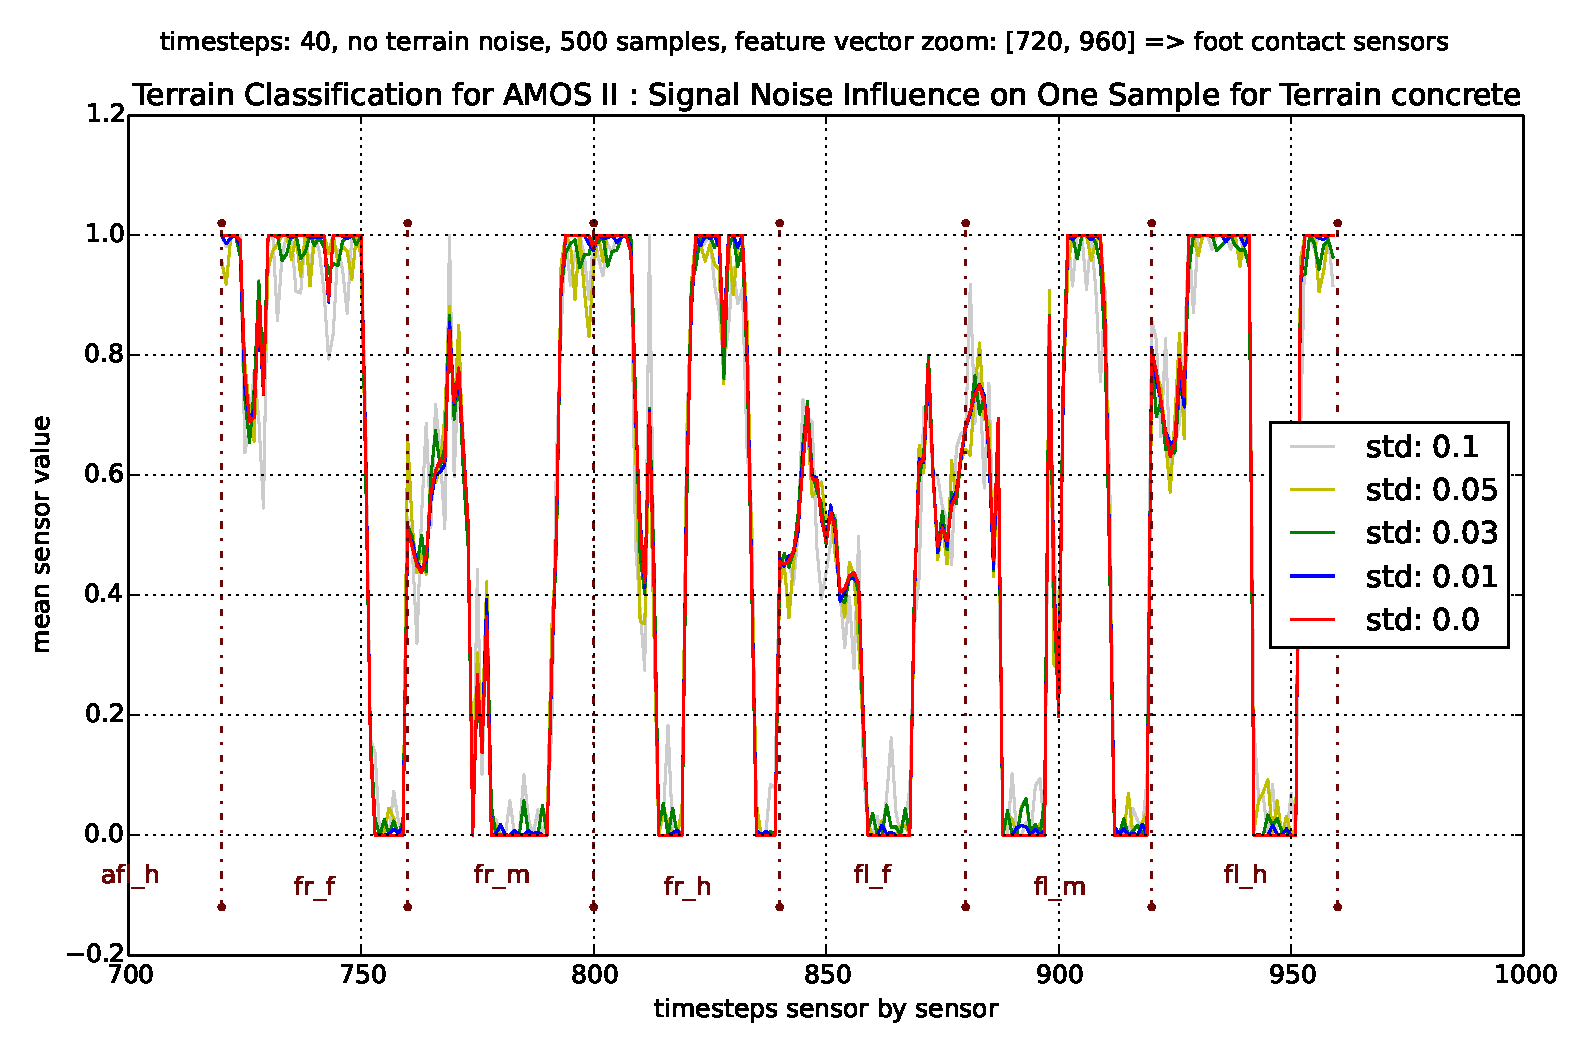
\includegraphics[width=1.0\textwidth]{sn_analysis_one_sample_40_angle_concrete}
  \caption{Signal noise influence on one sample, terrain: concrete, angle sensors}
  \label{fig:sn_analysis_one_sample_angle_concrete}
\end{figure}

\begin{figure}[H]
  \centering
  \includegraphics[width=1.0\textwidth]{sn_analysis_one_sample_40_foot_contact_concrete}
  \caption{Signal noise influence on one sample, terrain: concrete, foot contact sensors}
  \label{fig:sn_analysis_one_sample_foot_contact_concrete}
\end{figure}

\begin{figure}[H]
  \centering
  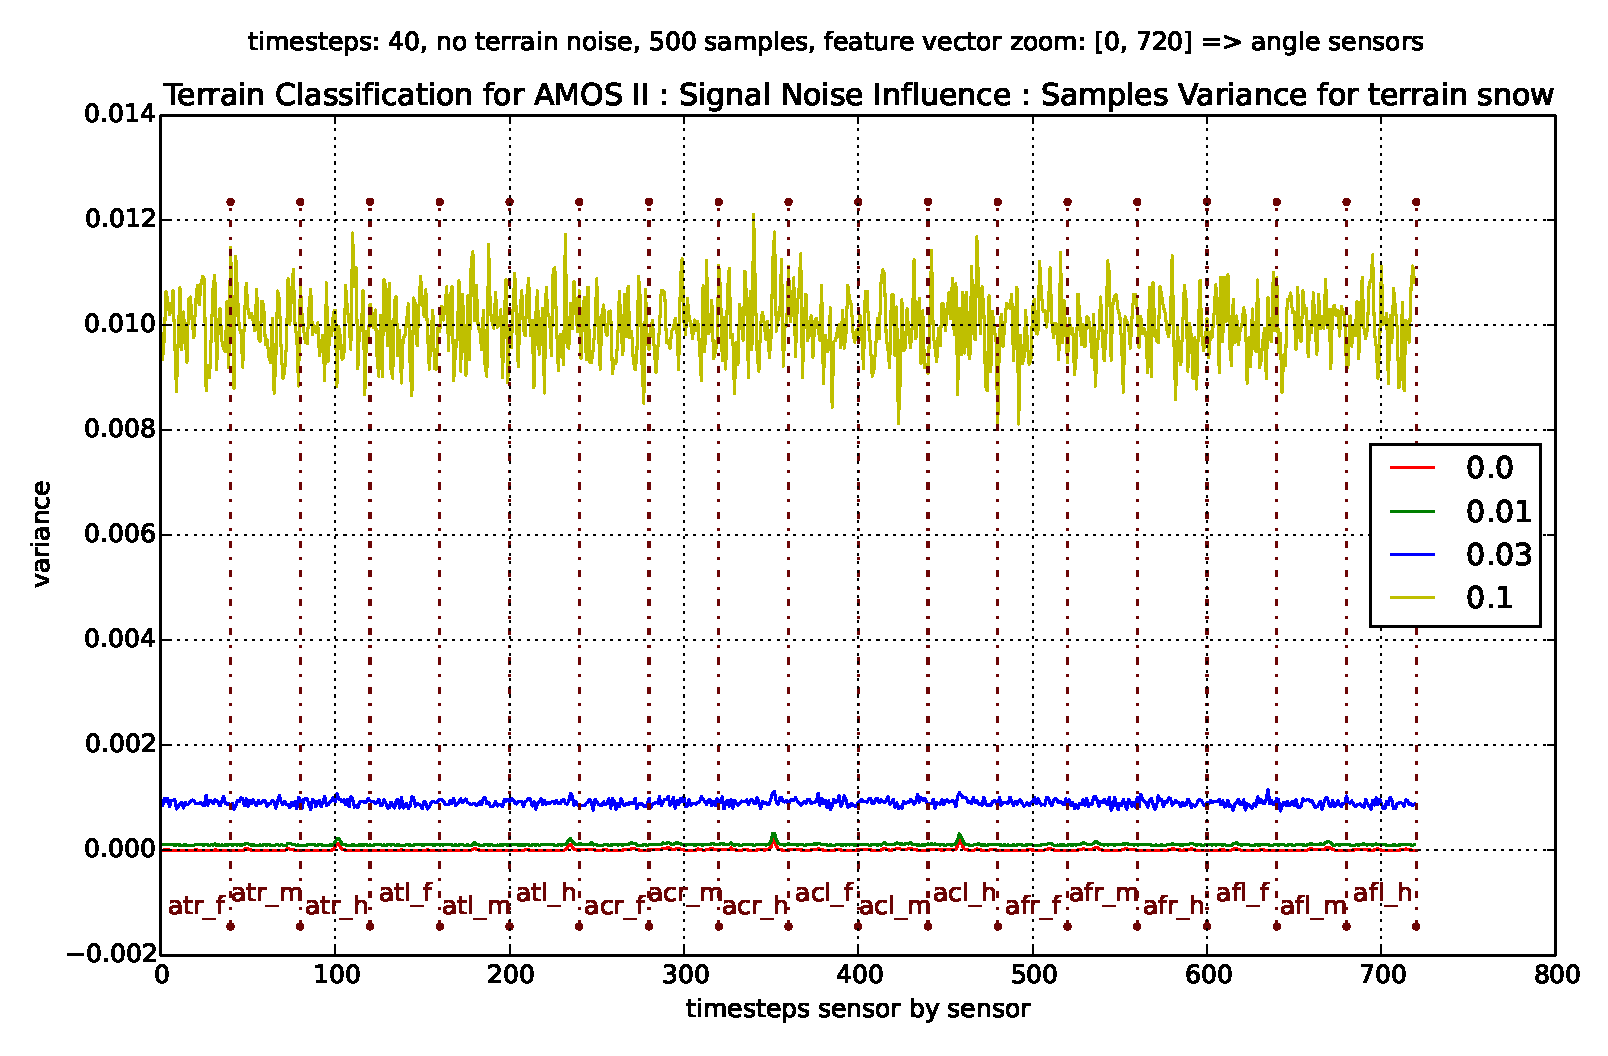
\includegraphics[width=1.0\textwidth]{sn_analysis_40_angle_snow}
  \caption{Signal noise analysis : samples variance, terrain: snow, angle sensors}
  \label{fig:sn_analysis_angle_snow}
\end{figure}

\begin{figure}[H]
  \centering
  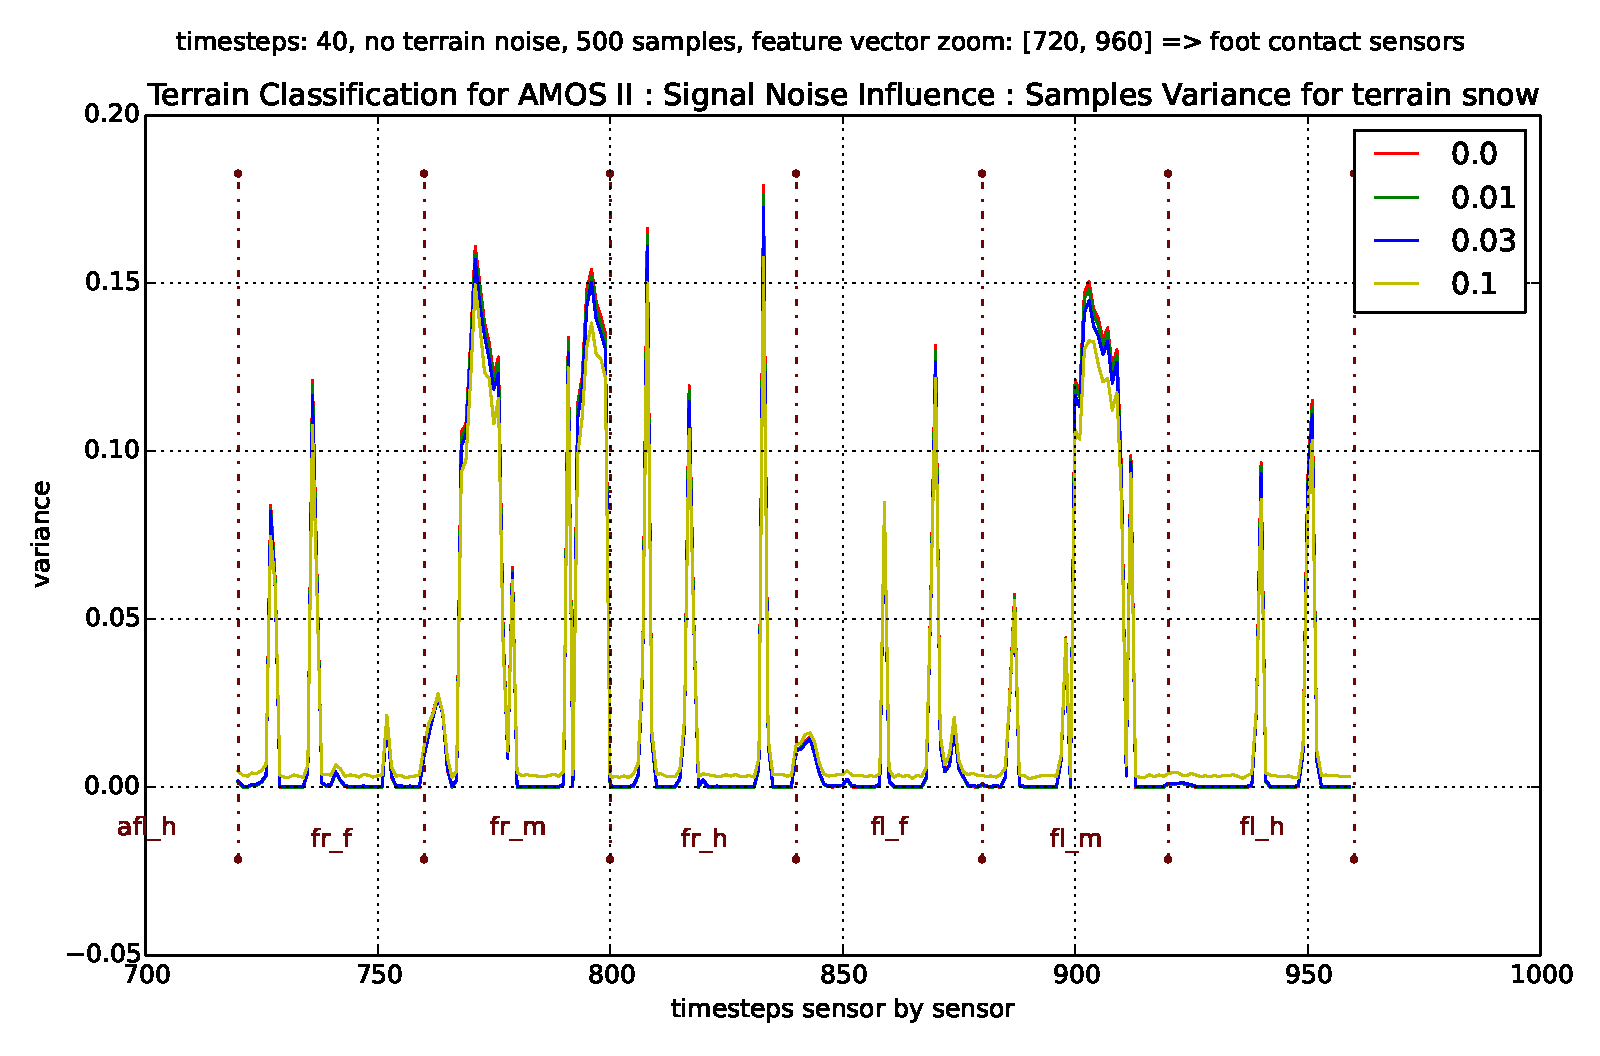
\includegraphics[width=1.0\textwidth]{sn_analysis_40_foot_contact_snow}
  \caption{Signal noise analysis : samples variance, terrain: snow, foot contact sensors}
  \label{fig:sn_analysis_foot_contact_snow}
\end{figure}

\subsection{Generated Datasets} \label{ssec:generated_datasets}

\begin{table}[H]
\centering
\caption{Generated datasets}
\label{tab:generated_datasets}
\begin{tabular}{|c|c|c|c|c|c|c|}
\hline
\multicolumn{1}{|l|}{\textit{name}} & \multicolumn{1}{l|}{\textit{ter. noise}} & \multicolumn{1}{l|}{\textit{sig. noise}} & \multicolumn{1}{l|}{\textit{timesteps}} & \multicolumn{1}{l|}{\textit{sensors}} & \multicolumn{1}{l|}{\textit{terrains}} & \multicolumn{1}{l|}{\textit{samples}} \\ \hline
ds\_01                              & 0.0                                             & 0.0                                            & 40                                      & all                                   & all                                    & 500                                     \\ \hline
ds\_02                              & 0.0                                             & 0.0                                            & 40                                      & angle                                 & all                                    & 500                                     \\ \hline
ds\_03                              & 0.0                                             & 0.0                                            & 40                                      & foot                                  & all                                    & 500                                     \\ \hline
ds\_04                              & 0.0                                             & 0.0                                            & 1                                       & all                                   & all                                    & 500                                     \\ \hline
ds\_05                              & 0.0                                             & 0.0                                            & 10                                      & all                                   & all                                    & 500                                     \\ \hline
ds\_06                              & 0.0                                             & 0.0                                            & 80                                      & all                                   & all                                    & 500                                     \\ \hline
ds\_07                              & 0.0                                             & 0.01                                           & 40                                      & all                                   & all                                    & 500                                     \\ \hline
ds\_08                              & 0.0                                             & 0.03                                           & 40                                      & all                                   & all                                    & 500                                     \\ \hline
ds\_09                              & 0.0                                             & 0.05                                           & 40                                      & all                                   & all                                    & 500                                     \\ \hline
ds\_10                              & 0.0                                             & 0.1                                            & 40                                      & all                                   & all                                    & 500                                     \\ \hline
ds\_11                              & 0.01                                            & 0.0                                            & 40                                      & all                                   & all                                    & 500                                     \\ \hline
ds\_12                              & 0.03                                            & 0.0                                            & 40                                      & all                                   & all                                    & 500                                     \\ \hline
ds\_13                              & 0.05                                            & 0.0                                            & 40                                      & all                                   & all                                    & 500                                     \\ \hline
ds\_14                              & 0.1                                             & 0.0                                            & 40                                      & all                                   & all                                    & 500                                     \\ \hline
ds\_15                              & 0.2                                             & 0.0                                            & 40                                      & all                                   & all                                    & 500                                     \\ \hline
\end{tabular}
\end{table}

\subsection{Classification results} \label{ssec:classification_results}

\begin{table}[H]
\centering
\caption{Classification results}
\label{tab:classification_results}
\begin{tabular}{|c|c|c|c|c|c|c|}
\hline
\multirow{2}{*}{\textit{dataset}} & \multicolumn{3}{c|}{\textit{\textbf{kitt net}}}         & \multicolumn{3}{c|}{\textit{\textbf{sknn net}}}         \\ \cline{2-7} 
                                  & \textit{accuracy} & \textit{precision} & \textit{recall} & \textit{accuracy} & \textit{precision} & \textit{recall} \\ \hline
ds\_01                            &                   &                    &                 &                   &                    &                 \\ \hline
ds\_02                            &                   &                    &                 &                   &                    &                 \\ \hline
ds\_03                            &                   &                    &                 &                   &                    &                 \\ \hline
ds\_04                            &                   &                    &                 &                   &                    &                 \\ \hline
ds\_05                            &                   &                    &                 &                   &                    &                 \\ \hline
ds\_06                            &                   &                    &                 &                   &                    &                 \\ \hline
ds\_07                            &                   &                    &                 &                   &                    &                 \\ \hline
ds\_08                            &                   &                    &                 &                   &                    &                 \\ \hline
ds\_09                            &                   &                    &                 &                   &                    &                 \\ \hline
ds\_10                            &                   &                    &                 &                   &                    &                 \\ \hline
ds\_11                            &                   &                    &                 &                   &                    &                 \\ \hline
ds\_12                            &                   &                    &                 &                   &                    &                 \\ \hline
ds\_13                            &                   &                    &                 &                   &                    &                 \\ \hline
ds\_14                            &                   &                    &                 &                   &                    &                 \\ \hline
ds\_15                            &                   &                    &                 &                   &                    &                 \\ \hline
\end{tabular}
\end{table}

\subsection{Final Configuration} \label{ssec:final_configuration}

\section{Pruning Algorithm Results} \label{sec:pruning_algorithm_results}

For instance, considering the MNIST dataset, there is an image (meaning a vector of pixels) as the network input. As the output, there are $ 10 $ classes corresponding to digits. Having the minimal structure, one can find out which pixels are related to e.g. digit $ 5 $ class and/or which pixels are totally useless for classification. This analysis is briefly presented in section X. 


evaluation (tables and figures) of classification:
\begin{itemize}
\item various terrain noise standard deviation values
\item various signal noise standard deviation values
\item various sensors on network input (only foot, only angle...)
\item various timesteps used as one sample (-> time needed for detection)
\item various number of detected terrains as outputs
\item various network structures
\item various training parameters (epochs, learning rate, batch size...)
\end{itemize}


evaluation of neural nets as a classifier:
\begin{itemize}
\item comparison to other classifiers on the same data, classifiers are ready provided by sknn library
\end{itemize}

evaluation of proprioception sensing against other methods (visual, haptic, laser...):
\begin{itemize}
\item comparison to the results from the literature
\end{itemize}

evaluation of the pruning algorithm:
\begin{itemize}
\item various starting structures, ends up with the same minimal-optimal structure?
\item various noise types, same minimal structure?
\item speed comparisons of the fully-connected vs. pruned structure
\item further analysis:
 \begin{itemize}
 \item which sensors are redundant/crucial
 \item which sensors are important for which terrain
 \item comments on the minimal structure and benefits of having it
 \end{itemize}
\end{itemize}
10-15 pages (many figures, tables)
